\begin{Indication}{1.1.1}
	Utiliser les propriétés de la fonction logarithme népérien : $\ln(a)+\ln(b)=\ln(b)$ , $\ln(a)-\ln(b)=\ln\left(\frac{a}{b}\right)$ et $\ln\left(a^b\right)=b\ln(a)$
\end{Indication}
\begin{Solution}{1.1.1}
\begin{enumerate}
	\item $A=10\ln(2) \quad B=6\ln(2) \quad C=-4\ln(2) \quad D=-\ln(2)$
	\item $A=-\ln(9) \quad B=0 \quad C=0 \quad D=6+2\ln(2)$
\end{enumerate}
\end{Solution}
\begin{Solution}{1.1.2}
	$A=0 \quad B=0 \quad C=\ln(x+1) \quad D=\ln(x+1) \quad E=0 \quad F=-\ln(n)$
\end{Solution}
\begin{Solution}{1.1.6}
\begin{tabular}{p{0.21\textwidth} p{0.38\textwidth} p{0.3\textwidth}}
	$S_1=\left\{\left(\ln(2);\ln(5)\right)\right\}$ & $S_2=\left\{\left(1+\sqrt{1+e^3};-1+\sqrt{1+e^3}\right)\right\}$ & $S_3=\left\{\left(3e^2;2e^3\right);\left(2e^3;3e^2\right)\right\}$\\
	$S_4=\left\{\left(\frac{1}{e};e^6\right)\right\}$ & $S_5=\left\{\left(e;\frac{1}{e}\right);\left(-e;\frac{-1}{e}\right)\right\}$
\end{tabular}
\end{Solution}
\begin{Indication}{1.1.7}
	Utiliser le changement de variable $X=\ln(x)$
\end{Indication}
\begin{Solution}{1.1.7}
	\begin{tabular}{p{0.4\textwidth} p{0.4\textwidth}}
		a) $S=\left\{1;e^{-2}\right\}$ & b) $S=\left]e^{-2};e\right[$ \\
		c) $S=]1;e[$ & d) $S=\left]0;e^{-\frac{1}{2}}\right]\cup]1;+\infty[$\\
		e) $S=\left[e^{-3};e^4\right]$ & f) $S=\left\{e^{-1};e^{-e}\right\}$
    \end{tabular}
\end{Solution}
\begin{Indication}{1.1.8}
	Résoudre l'équation en composant chaque membre par la fonction logarithme.
\end{Indication}
\begin{Solution}{1.1.8}
	$S=\{0;1;4\}$
\end{Solution}
\begin{Indication}{1.2.3}
	\begin{enumerate}
		\item Exprimer $v_{n+1}$ en fonction de $v_n$ et repérer une identité remarquable.
		\item Exprimer $v_n$ en fonction de $n$ puis $u_n$ en fonction de $v_n$
	\end{enumerate}
\end{Indication}
\begin{Solution}{1.2.3}
	2. $u_n=\frac{1-2^{2^{n+1}}}{3}$
\end{Solution}
\begin{Indication}{1.3.1}
	\begin{enumerate}
		\item Appliquer la fonction logarithme sur chaque membre de l'inégalité.
		\item Utiliser $\left(\ln(x)\right)'=\frac{1}{x}$ et penser à calculer $f(3)$
		\item[4.] Utiliser les questions précédentes.
	\end{enumerate}
\end{Indication}
\begin{Solution}{1.3.1}
	\begin{enumerate}
		\item[2.] La valeur de $f\left(\frac{3}{\ln(3)}\right)$ est approchée à $10^{-3}$\\
		\begin{tikzpicture}
			\tkzTabInit[espcl=5pt]{$x$/1,$f'(x)$/1,$f(x)$/2}{$0$,$\frac{\ln(3)}{3}$,$+\infty$}
			\tkzTabLine {d , + , z , -}				
			\tkzTabVar {D-/, +/{$0,015$} , -/}
            \tkzTabVal{2}{3}{0.5}{$3$}{$0$}
		\end{tikzpicture}
	\end{enumerate}
\end{Solution}
\begin{Indication}{1.3.2}
	Il s'agit d'une fonction composée, commencer par déterminer sous quelles conditions le logarithme peut exister, puis s'intéresser à la racine carrée.
\end{Indication}
\begin{Solution}{1.3.2}
	$\Dcal_g=\emptyset$
\end{Solution}
\begin{Indication}{1.3.3}
	\begin{enumerate}
		\item Dresser le tableau de variations de la fonction $f:x\mapsto x-\ln(1+x)$ sur $]1;+\infty[$
		\item Dresser le tableau de variations de la fonction $g:x\mapsto x-\frac{x^2}{2}-\ln(1+x)$ sur $[0;+\infty[$
	\end{enumerate}
\end{Indication}
\begin{Solution}{1.3.3}
	\begin{enumerate}
		\item $f'(x)=\frac{x}{1+x}$, on a donc le tableau suivant :\\
		\begin{tikzpicture}
			\tkzTabInit[espcl=5pt]{$x$/1 , $f'(x)$/1 , $f(x)$/2}{$-1$ , $0$ , $+\infty$}
			\tkzTabLine {d , - , z , +}
			\tkzTabVar {D+/ , -/$0$ , +/}
		\end{tikzpicture}
		
		On voit que $f(x)\geq0$ sur $]1;+\infty[$, ce qui conclut notre preuve.
		\item $g'(x)=\frac{x^2}{1+x}$, on a donc le tableau suivant :\\
		\begin{tikzpicture}
			\tkzTabInit[espcl=5pt]{$x$/1 , $g'(x)$/1 , $g(x)$/2}{$0$ , $+\infty$}
			\tkzTabLine { , - , }
			\tkzTabVar {+/0 , -/}
		\end{tikzpicture}
		
		On voit que $g(x)\leq0$ sur $[0;+\infty[$, ce qui conclut notre preuve.
	\end{enumerate}
\end{Solution}
\begin{Indication}{1.3.7}
On pourra étudier les variations de la fonction $x:\mapsto\ln(x)+\frac{1}{x}$
\end{Indication}
\begin{Solution}{1.3.7}
	$\Dcal_f=\RR_+^*$ et on a $f'(x)=e^x\left(\frac{1}{x}+\ln(x)\right)=e^xg(x)$
	
	Or $g'(x)=\frac{x-1}{x^2}$, on obtient donc le tableau suivant :\\
	\begin{tikzpicture}
		\tkzTabInit[espcl=5pt]{$x$/1 , $g'(x)$/1 , $g(x)$/2}{$0$ , $1$ , $+\infty$}
		\tkzTabLine {d , - , z , +}
		\tkzTabVar {D+/ , -/$1$ , +/}
	\end{tikzpicture}
	
	On voit que la fonction $g$ est strictement positive sur $\RR_+^*$, ce qui implique que $f'$ est strictement positive sur $\RR_+^*$, ainsi $f$ est strictement croissante sur son domaine de définition.
\end{Solution}
\begin{Indication}{1.3.8}
	\begin{enumerate}
		\item Déterminer l'équation réduite de la tangente à la courbe du logarithme en un point d'abscisse $a>0$, puis injecter les coordonnées du point $(0;1)$
		\item Déterminer l'équation réduite de la tangente à $\Ccal_f$ en un point d'abscisse $a>0$ puis injecter les cordonnées de l'origine du repère/
	\end{enumerate}
\end{Indication}
\begin{Solution}{1.3.8}
	\begin{enumerate}
		\item Au point $A\left(e^2;2\right)$, la tangente à la courbe du logarithme est $T:y=\frac{x}{e^2}+1$ et passe bien par le point de coordonnées $(0;1)$
		\item Au point $B\left(e^{\frac{1}{2}};\frac{e^{-\frac{1}{2}}}{2}\right)$, la tangente à $\Ccal_f$ est $T:y=\frac{x}{2e}$ et passe bien par l'origine du repère.
	\end{enumerate}
\end{Solution}
\begin{Indication}{1.3.9}
	\begin{enumerate}
		\item[3.] Rappeler que le coefficient directeur de la tangente à $\Ccal_f$ est donné par $f'(x)$ puis utiliser le changement de variable $X=\ln(x)$
		\item[4.] Rappeler que le coefficient directeur de la tangente à $\Ccal_f$ est donné par $f'(x)$ puis utiliser le changement de variable $X=\ln(x)$
	\end{enumerate}
\end{Indication}
\begin{Solution}{1.3.9}
	\begin{enumerate}
		\item[2.] $f'(x)=\frac{\ln(x)-1}{\ln(x)^2}$, on a donc le tableau suivant :\\
		\begin{tikzpicture}
			\tkzTabInit[espcl=5pt] {$x$ /1 , $f'(x)$ /1 , $f(x)$/2}{$0$ , $1$ , $e$ , $+\infty$}
			\tkzTabLine {d , - , d , - , z , +}
			\tkzTabVar {D+/ , D+/ , -/$e$ ,+/}
		\end{tikzpicture}
		\item[3.] On cherche à résoudre l'équation $f'(x)=2$, ce qui équivaut à $2\ln^2(x)-\ln(x)+1=0$\\
		On pose alors $X=\ln(x)$ et on voit que cette équation n'a pas de solution.
		\item[4.] On cherche à résoudre l'équation $f'(x)=-2$, ce qui équivaut à $2\ln^2(x)+\ln(x)-1=0$\\
		On pose alors $X=\ln(x)$, et on obtient après résolution de l'équation $x=\sqrt{e}$ ou $x=\frac{1}{e}$\\
		On donne alors l'équation des tangentes à $\Ccal_f$ aux points d'abscisse trouvées : $T_1:y=-2x+\frac{1}{e}$ et $T_2:y=-2x+4\sqrt{e}$
	\end{enumerate}
\end{Solution}
\begin{Indication}{1.3.10}
	\begin{enumerate}
	\item[2.] Écrire $P(x)=ax^2+bx+c$ puis déterminer les valeurs de $a$, $b$ et $c$ pour que les expressions soient égales.
	\end{enumerate}
\end{Indication}
\begin{Solution}{1.3.10}
	\begin{enumerate}
		\item $h'(x)=1-\frac{3x^2}{2+x^3}$
		\item $P(x)=x^2-2x-2$
		\item \begin{tikzpicture}
			\tkzTabInit {$x$/1 , $h'(x)$/1 , $h(x)$/2} {$-1$ , $1-\sqrt{3}$ , $1$ , $1+\sqrt{3}$ , $+\infty$}
			\tkzTabLine {, - , z , + , z , - , z , + , }
			\tkzTabVar {+/{$-1$} , -/{$-1,207$} , +/{$-0,099$} , -/{$-0,377$} , +/}
		\end{tikzpicture}
	\end{enumerate}
\end{Solution}
\begin{Solution}{1.3.11}
	\begin{tikzpicture}
		\tkzTabInit {$x$/1 , $\phi'(x)$/1 , $\phi(x)$/2} {$-\infty$ , $-\sqrt{e-1}$ , 0 , $\sqrt{e-1}$ , $+\infty$}
		\tkzTabLine { , + , z , - , z , + , z}
		\tkzTabVar {-/ , +/{$\frac{1}{e}$} , -/0 , +/{$\frac{1}{e}$} , -/}
	\end{tikzpicture}
	\vspace{10pt}
\end{Solution}
\begin{Indication}{1.3.12}
	\begin{enumerate}
		\item[3.] Utiliser le signe des fonctions $f$ et $g$
		\item[4.] Poser $X=\frac{1+x}{x}$
		\item[5.] Utiliser les propriétés de la fonction logarithme.
	\end{enumerate}
\end{Indication}
\begin{Solution}{1.3.12}
	\begin{enumerate}
	\begin{minipage}{0.45\linewidth}
	\item \begin{tikzpicture}
			\tkzTabInit[espcl=2.5pt] {$x$/1 , $f'(x)$/1 , $f(x)$/2} {$0$ , $1$ , $+\infty$}
			\tkzTabLine {d , + , z , -}
			\tkzTabVar {D-/ , +/$0$ , -/}
		\end{tikzpicture}
	\end{minipage}\hfill
	\begin{minipage}{0.45\linewidth}
	\item \begin{tikzpicture}
			\tkzTabInit[espcl=2.5pt] {$x$/1 , $g'(x)$/1 , $g(x)$/2} {$0$ , $1$ , $+\infty$}
			\tkzTabLine {d , + , z , -}
			\tkzTabVar {D-/ , +/$0$ , -/}
		\end{tikzpicture}
	\end{minipage}
	\item $f(x)\leq0$ donc $\ln(x)\leq x-1$ sur $\RR^*_+$\\
	$g(x)\leq0$ donc $\ln(x)\geq \frac{x-1}{x}$ sur $\RR^*_+$\\
	On a bien les deux inégalités demandées.
	\item Pour $\xR^*_+$ on pose $X=\frac{1+x}{x}$. Alors $X\in\RR^*_+$. Donc d'après la question 3. on a :\\
	$\frac{X-1}{X}\leq\ln(X)\leq X-1$.\\
	En remplaçant dans ces inégalités $X$ par $\frac{1+x}{x}$ et en simplifiant, on obtient bien $\frac{1}{x+1}\leq\ln\left(\frac{1+x}{x}\right)\leq\frac{1}{x}$
	\item $\ln\left(\frac{2}{1}\right)+\ln\left(\frac{3}{2}\right)+\ln\left(\frac{4}{3}\right)+\ldots+\ln\left(\frac{1+n}{n}\right) = \ln(1+n)$
	\item D'après la question 4. pour tout $k\in\NN$ on peut affirmer que $\frac{1}{k+1}\leq\ln\left(\frac{1+k}{k}\right)$, ainsi :\\
	$\frac{1}{2}+\frac{1}{3}+\frac{1}{4}+\ldots+\frac{1}{n+1}\leq\ln\left(\frac{2}{1}\right)+\ln\left(\frac{3}{2}\right)+\ln\left(\frac{4}{3}\right)+\ldots+\ln\left(\frac{1+n}{n}\right)=\ln(1+n)$
	\end{enumerate}
\end{Solution}
\begin{Indication}{1.3.13}
	\begin{enumerate}
		\item[2.] Exprimer $f(x)$ en fonction de $g(x)$
	\end{enumerate}
\end{Indication}
\begin{Solution}{1.3.13}
	\begin{enumerate}
		\item \begin{tikzpicture}
			\tkzTabInit[espcl=5pt] {$x$/1 , $g'(x)$/1 , $g(x)$/2} {$0$ , $1$ , $+\infty$}
			\tkzTabLine {d , - , z , + , }
			\tkzTabVar {D+/ , -/1 , +/}
		\end{tikzpicture}
		\item $g$ est positive sur $\RR^*_+$ et $f(x)=\frac{g(x)}{x^2}$ donc $f$ est positive sur $\RR^*_+$
		\item \begin{enumerate}
			\item $\Acal_{MPOQ}=af(a)$
			\item En posant $\Acal(a)=af(a)$, on obtient $\Acal'(a)=\frac{a-2}{a^2}$\\
			On peut alors dresser le tableau de variations de $\Acal$ et on voit que son minimum est atteint en $a=2$, Or $\Acal(2)=\ln(2)$
		\end{enumerate}		
	\end{enumerate}
\end{Solution}
\begin{Solution}{2.1.1}
\renewcommand{\arraystretch}{2}
	\begin{tabular}{p{0.3\linewidth}p{0.3\linewidth}p{0.3\linewidth}}
	$f_1'(x)=\frac{2x+3x^2}{\sqrt{1+x^2+x^3}}$ & $f_2'(x)=\left(1-\frac{1}{x^2}\right)e^{x+\frac{1}{x}}$ & $f_3'(x)=\left(14-7e^x\right)(2x-e^x)^6$ \\
	$f_4'(x)=\frac{3-4x\sqrt{x}}{6x-2x^2\sqrt{x}}$ & $f_5'(x)=-\frac{4\left(6-\ln(x)\right)^3}{x}$ & $f_6'(x)=\left(2x^2+1\right)e^{x^2}$ \\
	$f_7'(x)=e^{x\ln(x)}(1+\ln(x))-7$ & $f_8'(x)=(2x^2+2x-2)e^{3+2x}$ & $f_9'(x)=\frac{4x^2+3x+2}{\sqrt{1+x^2}}$ \\	
	$f_{10}'(x)=\frac{12x^2-4x-6}{x^{x^2+1}}$ & $f_{11}'(x)=\frac{15x^2+3x+1}{(10x+4)\sqrt{5x+2}}$ & $f_{12}'(x)=\frac{(2x^2+4x+3)e^x}{(2x+3)\sqrt{2x+3}}$ \\
	$f_{13}'(x)=8xe^{1+x^2}\left(1+e^{1+x^2}\right)^{3}$ & $f_{14}'(x)=\frac{2x-1}{x(2x-2)\sqrt{\ln(x-x^2}}$ & $f_{15}'(x)=\frac{e^{\sqrt{1+\ln(x)}}}{2x\sqrt{1+\ln(x)}}$
\end{tabular}
\end{Solution}
\begin{Solution}{2.1.2}
\begin{minipage}{0.45\linewidth}
	\begin{tikzpicture}
		\tkzTabInit[espcl=1.75]{$x$ /1, $f(x)$ /2}{$-\infty$ , $-1$ , $1$ , $+\infty$}
		\tkzTabVar{+/, -D+/ , -/$\frac{\sqrt{2}}{2}$,+/}
	\end{tikzpicture}
	
	\begin{tikzpicture}
		\tkzTabInit{$x$ /1, $h(x)$ /2}{$0$ , $\frac{4}{49}$ , $+\infty$}
		\tkzTabVar{-/$0$ , +/$\frac{4\times5^5}{7^7}$, -/}
	\end{tikzpicture}
\end{minipage}\hfill
\begin{minipage}{0.45\linewidth}
	\begin{tikzpicture}
		\tkzTabInit{$x$ /1, $g(x)$ /2}{$0$,$\frac{1}{4}$,$+\infty$}
		\tkzTabVar{-/$0$ , +/$\frac{1}{2}e^{\frac{1}{2}}$, -/}
	\end{tikzpicture}
	
	\begin{tikzpicture}
		\tikzset{h style/.style = {pattern=north west lines}}
		\tkzTabInit[espcl=1.75]{$x$ /1, $\rho(x)$ /2}{$-\infty$,$-2$,$0$,$+\infty$}
		\tkzTabVar{-/ , +H/$0$ / , -/$0$ / , +/ }
	\end{tikzpicture}
\end{minipage}
\vspace{10pt}
\end{Solution}
\begin{Solution}{2.1.3}
	\begin{tabular}{p{0.23\linewidth}p{0.23\linewidth}p{0.18\linewidth}p{0.25\linewidth}}
		$f_1''(x)=20x^3-24x^2+2$ & $f_2''(x)=(x^2+4x+2)e^x$ & $f_3''(x)=\frac{2}{x^3}$ & $f_4''(x)=\frac{3x-1}{4x\sqrt{x}}$\\
		$f_5''(x)=2x(2x^3+3)e^{x^2}$ & $f_6''(x)=\frac{-1}{(1-x^2)\sqrt{1-x^2}}$ & $f_7''(x)=\frac{e^{\sqrt{x}}(\sqrt{x}-1)}{4x\sqrt{x}}$ & $f_8''(x)=\frac{4x^2-12x+3}{\sqrt{x}e^x}$
	\end{tabular}
\end{Solution}
\begin{Solution}{2.1.4}
	$f''(x)=a^2e^{ax+b} > 0$, donc $f$ est convexe.\\
\end{Solution}
\begin{Indication}{2.1.5}
	\begin{enumerate}
		\item Utiliser une définition de la convexité.
		\item Utiliser le fait que $[AB]$ est une corde de $\Ccal_g$
		\item[4.] Reprendre les questions précédentes
	\end{enumerate}
\end{Indication}
\begin{Solution}{2.1.5}
	\begin{enumerate}
		\item $g'(x)=e^x$ donc $g'$ est croissante, donc $g$ est convexe.
		\item $\Ccal_g$ est en-dessous de $(AB)$ sur $[0;1]$, et au-dessus sinon.
		\item $(AB):y=(e-1)x+1$
		\item $e^x+x\geq1+ex \Leftrightarrow e^x\geq(e-1)x+1$ donc $S=]-\infty;0]\cup[1;+\infty[$
	\end{enumerate}
\end{Solution}
\begin{Indication}{2.1.6}
	\begin{enumerate}
		\item[3.] Utiliser la formule des coordonnées du milieu d'un segment.
		\item[4.] Comparer leurs ordonnées grâce à la convexité de $f$
		\item[5.] reprendre les deux questions précédentes.
	\end{enumerate}
\end{Indication}
\begin{Solution}{2.1.6}
	\begin{enumerate}
	\begin{minipage}{0.5\linewidth}
		\item 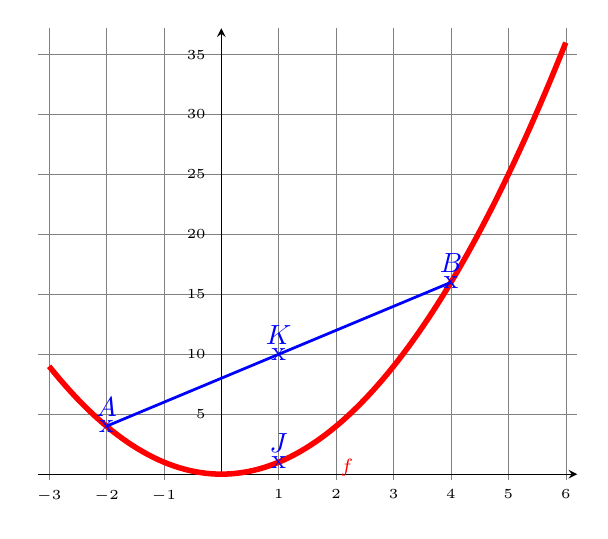
\begin{tikzpicture}
    		\begin{axis}[xmin = -3, xmax = 6, ymin = 0, ymax = 37,
    		xtick distance=1, ytick distance=5, grid = major,
       		major grid style = {line width = 0.2pt , draw = gray},
        	axis lines = middle, enlargelimits = { abs = 0.2 },
        	ticklabel style = {font = \tiny }]
    			\addplot[line width = 2pt , domain=-3:6, samples=100, color=red]
    			{x^2};
    			\node[color=red] at (2.2,0.5) {$\Ccal_f$};
    			\draw[color=blue,line width=1pt] (-2,4)--(4,16);
    			\draw[color=blue] node[above] at (-2,4) {$A$};
    			\draw[color=blue] node at (-2,4) {x};
    			\draw[color=blue] node[above] at (4,16) {$B$};
    			\draw[color=blue] node at (4,16) {x};
    			\draw[color=blue] node[above] at (1,1) {$J$};
    			\draw[color=blue] node at (1,1) {x};
    			\draw[color=blue] node[above] at (1,10) {$K$};
    			\draw[color=blue] node at (1,10) {x};
    		\end{axis}
    	\end{tikzpicture}
    	\end{minipage}
    	\begin{minipage}{0.5\linewidth}
    	\item $y_A=a^2 \quad y_B=b^2 \quad y_J=\frac{(a+b)^2}{4}$\\
    	\item $x_K=\frac{a+b}{b} \quad y_K=\frac{a^2+b^2}{2}$\\
    	\item La fonction $f$ est convexe, $J$ et $K$ ont la même abscisse mais $K$ se situe sur une corde de $\Ccal_f$ alors que $J$ se situe sur $\Ccal_f$. On en déduit donc que l'ordonnée de $K$ est supérieure à celle de $J$\\
    	\item En reprenant les questions 3. et 4. on obtient $\frac{a^2+b^2}{2}\geq\frac{(a+b)^2}{4}$ donc $(a+b)^2\leq2(a^2+b^2)$\\
    	En développant l'identité remarquable ci-dessus on obtient rapidement que $a^2+b^2\geq2ab$
    	\end{minipage}
	\end{enumerate}
\end{Solution}
\begin{Indication}{2.1.7}
Essayer de trouver des contre-exemples pour les propositions qui semblent fausses.\\
Pour celles qui sont vraies,  une démonstration est requise, notamment en dérivant deux fois les fonctions proposées pour étudier leur convexité.
\end{Indication}
\begin{Solution}{2.1.7}
	1. Vrai \qquad 2. Vrai \qquad 3. Faux \qquad 4. Faux \qquad 5. Vrai \qquad 6. Faux\\
\end{Solution}
\begin{Indication}{2.2.1}
Dériver deux fois la fonction $f$ puis étudier le signe de $f''$. Penser à donner l'ordonnée des points d'inflexion.
\end{Indication}
\begin{Solution}{2.2.1}
$f''(x)=12(x^2+x-2)$\\
On résout l'inéquation $f''(x)\geq0$ par discriminant et on obtient que $f$ est concave sur $[-2,1]$ et convexe sur $]-\infty;-2]\cup[1;+\infty[$\\
Ses points d'inflexions sont $A(-2;-68)$ et $B(1;-11)$
\end{Solution}
\begin{Solution}{2.2.2}
\begin{minipage}{0.5\linewidth}
$\varphi'(x)=\frac{x-1}{2x\sqrt{x}}$ et $\varphi''(x)=\frac{3-x}{4x^2\sqrt{x}}$\\
On dresse le tableau de variations de $\varphi$ :

\begin{tikzpicture}
	\tkzTabInit{$x$ /1, $\varphi(x)$ /2}{$0$,$1$,$+\infty$}
	\tkzTabVar{D+/ , -/$2$, +/}
\end{tikzpicture}
\end{minipage}
\begin{minipage}{0.5\linewidth}
$\varphi$ est convexe sur $]0;3]$  et concave sur $[3;+\infty[$\\
$\Ccal_\varphi$ admet pour point d'inflexion $M\left(3;\frac{4}{\sqrt{3}}\right)$\\
\end{minipage}
\end{Solution}
\begin{Indication}{2.2.3}
	\begin{enumerate}
		\item Étudier le signe de $\mu'$
		\item Penser à utiliser la fonction logarithme pour résoudre l'inéquation $\mu(x)\geq0$
	\end{enumerate}
\end{Indication}
\begin{Solution}{2.2.3}
\begin{enumerate}
	\item $\mu'(x)=2e^{2x-1}+3e^{-3x}>0$, donc $\mu$ est bien strictement croissante sur $\RR$
	\item $\mu''(x)4e^{-2x-1}-9e^{-3x}$\\
	Ainsi $\mu''(x)\geq0\Leftrightarrow 4e^{2x-1}\geq9e^{-3x}\Leftrightarrow \ln\left(4e^{2x-1}\right)\geq\ln\left(9e^{-3x}\right)\Leftrightarrow \ln(4)+2x-1\geq\ln(9)-3x\Leftrightarrow x\geq\frac{1+\ln\left(\frac{9}{4}\right)}{5}$\\
	$\mu$ est donc convexe sur $\left[\frac{1+\ln\left(\frac{9}{4}\right)}{5};+\infty\right[$ et concave sur $\left]-\infty;\frac{1+\ln\left(\frac{9}{4}\right)}{5}\right]$
\end{enumerate}
\end{Solution}
\begin{Indication}{2.2.4}
	\begin{enumerate}
		\item Calculer $h(-x)$
		\item Étudier le signe de $h'$
		\item Développer le membre de droite puis identifier les coefficients.
		\item Étudier le signe de $h''$ à l'aide de la question 3.
	\end{enumerate}
\end{Indication}
\begin{Solution}{2.2.4}
	\begin{enumerate}
		\item $h(-x)=-xe^{-x^2}=-h(x)$, donc $h$ est impaire.
		\item $h'(x)=(1-2x^2)e^{-x^2}$, on obtient alors le tableau de variations suivant :
		
		\begin{tikzpicture}
			\tkzTabInit {$x$/1 , $h'(x)$/1 , $h(x)$/2} {$-\infty$ , $-\frac{\sqrt{2}}{2}$ , $\frac{\sqrt{2}}{2}$ , $+\infty$}
			\tkzTabLine {,- , z , + , z , -}
			\tkzTabVar {+/ , -/$-\frac{1}{e^{\frac{1}{2}}\sqrt{2}}$ , +/ $\frac{1}{e^{\frac{1}{2}}\sqrt{2}}$ , -/}
		\end{tikzpicture}
		\item $h''(x)=(4x^2-6)xe^{-x^2}$
		\item On obtient le tableau de convexité suivant :
		
		\begin{tikzpicture}
			\tkzTabInit {$x$/1 , $h''(x)$/1 , $h(x)$/1} {$-\infty$ , $-\sqrt{\frac{3}{2}}$ , $0$ , $\sqrt{\frac{3}{2}}$ , $+\infty$}
			\tkzTabLine {,-,z,+,z,-,z,+}
			\tkzTabLine {, \text{Concave} , , \text{Convexe} , , \text{Concave} , , \text{Convexe}}
		\end{tikzpicture}
	\end{enumerate}
\end{Solution}
\begin{Indication}{2.3.1}
	\begin{enumerate}
		\item Utiliser la formule $T_a:y=f'(a)(x-a)+f(a)$
		\item Montrer que $f''$ est positive.
		\item Utiliser la position des tangentes par rapport à la courbe d'une fonction concave.
	\end{enumerate}
\end{Indication}
\begin{Solution}{2.3.1}
	\begin{enumerate}
		\item $T_1:y=\frac{1}{2}x+\frac{1}{2}$
		\item $f''(x)=\frac{-1}{4x\sqrt{x}}<0$, donc $f$ est concave sur $\RR_+$
		\item $\Ccal_f$ est en dessous de $T_1$ sur $\RR_+$, on peut donc affirmer que $\sqrt{x}\leq\frac{1}{2}x+\frac{1}{2}$, ce qui revient à dire que $x\geq2\sqrt{x}-1$
	\end{enumerate}
\end{Solution}
\begin{Indication}{2.3.2}
	\begin{enumerate}
	\item Montrer que $f''$ est positive sur $\RR$
	\item Utiliser la formule $T_a:y=f'(a)(x-a)+f(a)$
	\item Utiliser la position des tangentes par rapport à la courbe d'une fonction convexe.
	\end{enumerate}
\end{Indication}
\begin{Solution}{2.3.2}
	\begin{enumerate}
		\item $g''(x)=e^x+4e^{-2x}>0$ donc $g$ est convexe sur $\RR$
		\item $T_0:y=-x+2$
		\item $\Ccal_f$ se situe au-dessus de $T_0$ sur $\RR$. On peut donc affirmer que $e^x+e^{-2x}\geq-x+2$ ce qui revient à dire que $e^x\geq2-x-e^{-2x}$
	\end{enumerate}
\end{Solution}
\begin{Indication}{2.3.3}
	\begin{enumerate}
		\item Montrer que $g'$ est strictement positive.
		\item Étudier le signe de $g''$
		\item Utiliser la formule $T_a:y=f'(a)(x-a)+f(a)$
		\item Utiliser que $(\Delta)$ est la tangente ) à $\Ccal_g$ en son unique point d'inflexion.
	\end{enumerate}
\end{Indication}
\begin{Solution}{2.3.3}
	\begin{enumerate}
		\item $g'(x)=e^x+e^{-x}>0$ donc $g$ est strictement croissante sur $\RR$
		\item $g''(x)=e^x-e^{-x}$\\
		Ainsi $g''(x)\geq0 \Leftrightarrow e^x\geq x^{-x} \Leftrightarrow x\geq0$\\
		$g$ est donc concave sur $\RR_-$ et convexe sur $\RR_+$
		\item $(\Delta):y=2x$
		\item Comme $(\Delta)$ est une tangente à $\Ccal_g$ en son unique point d'inflexion, on peut affirmer qu'elle se situe au-dessus de $\Ccal_g$ sur $\RR_-$ et en-dessous sur $\RR_+$\\
		De plus, $e^x\leq2x+e^{-x} \Leftrightarrow g(x)\leq2x$\\
		On obtient alors $S=\RR_-$
	\end{enumerate}
\end{Solution}
\begin{Indication}{2.3.5}
	\begin{enumerate}
		\item Montrer que $\varphi'(x)=P(x)e^{-x}$ où $P$ est un polynôme du second degré.
		\item Même indication que pour la question 1.
		\item Utiliser la formule $T_a:y=f'(a)(x-a)+f(a)$
		\item Utiliser la position relative de $\mathcal{T}_0$ et de $\Ccal_\varphi$ à l'aide de la convexité de la fonction $\varphi$
		\item[6.] Faire l'union des intervalles donnés dans les questions 4. et 5.
	\end{enumerate}
\end{Indication}
\begin{Solution}{2.3.5}
	\begin{enumerate}
		\item $\varphi'(x)=e^{-x}(x^2-4x+2)$, on obtient donc le tableau de variations suivant :
		
		\begin{tikzpicture}
			\tkzTabInit {$x$/1 , $\varphi'(x)$/1 , $\varphi(x)$/2} {$-\infty$ , $2-\sqrt{2}$ ,$2+\sqrt{2}$ , $+\infty$}
			\tkzTabLine {,+ , z , - , z , +}
			\tkzTabVar {-/ , +/{$0,461$} , -/{$-0,159$} , +/}
		\end{tikzpicture}
		\item $\varphi''(x)=e^{-x}(-x^2+6x-6)$, on obtient donc le tableau de convexité suivant :
		
		\begin{tikzpicture}
			\tkzTabInit {$x$/1 , $\varphi''(x)$/1 , $\varphi(x)$/2} {$-\infty$ , $3-\sqrt{3}$ ,$3+\sqrt{3}$ , $+\infty$}
			\tkzTabLine {,- , z , + , z , -}
			\tkzTabLine {,\text{Concave} , z , \text{Convexe} , z , \text{Concave}}
		\end{tikzpicture}
		\item $\mathcal{T}_0:y=2x$
		\item Comme $\varphi$ est concave sur $I=]-\infty;3-\sqrt{3}]$, on peut affirmer que $\Ccal_\varphi$ est en-dessous de $\mathcal{T}_0$ sur $I$.\\
		Or $\varphi(x)\leq2x \Leftrightarrow 2x(e^{-x}-1)\leq x^2e^{-x}$
		\item Si $x\geq1$, alors $e^{-x}\leq \frac{1}{e}$\\
		Ainsi $x\geq1 \Rightarrow \varphi(x)\leq\frac{2x-x^2}{e} \Rightarrow \varphi(x)\leq 2x$
		\item D'après la question 5. on peut affirmer que $\Ccal_\varphi$ est en dessous de $\mathcal{T}_0$ sur $J=[1;+\infty[$\\
		Ainsi $\Ccal_\varphi$ est en dessous de $\mathcal{T}_0$ sur $I\cup J=\RR$\\
		On peut donc affirmer que $2x(e^{-x}-1)\leq x^2e^{-x}$ sur $\RR$
	\end{enumerate}
\end{Solution}
\begin{Indication}{2.3.6}
	\begin{enumerate}
		\item[5.] Utiliser la formule $T_a:y=f'(a)(x-a)+f(a)$
		\item[6.] Raisonner sur $[-1;+\infty[$ puis sur $]-\infty;-1]$
	\end{enumerate}
\end{Indication}
\begin{Solution}{2.3.6}
	\begin{enumerate}
		\item $1+x^2>0$ donc $k$ est bien définie sur $\RR$. De plus $k$ est la composée du logarithme népérien et d'un polynôme qui sont deux fois dérivables, donc $k$ est deux fois dérivable.
		\item $k'(x)=\frac{2x}{1+x^2}$, on obtient donc le tableau de variations suivant :
		
		\begin{tikzpicture}
			\tkzTabInit {$x$/1 , $k'(x)$/1 , $k(x)$/2} {$-\infty$ , $0$ , $+\infty$}
			\tkzTabLine {,- , z , +}
			\tkzTabVar {+/ , -/$0$ , +/}
		\end{tikzpicture}
		\item[4.] $k''$ s'annule en $-1$ et en $1$ tout en changeant de signe, les points d'inflexion de $\Ccal_k$ sont donc $A(-1;\ln(2))$ et $B(1;\ln(2))$
		\item[5.] $T_1:y=x-1+\ln(2)$
		\item[6.] Comme $T_1$ est la tangente à $\Ccal_k$ en $B$, on peut affirmer qu'elle est au-dessus de $\Ccal_k$ sur $[1;+\infty[$ et en-dessous sur $[-1;1]$\\
		De plus, $k(x)\geq0$ et si $x\leq0$ alors $\Rightarrow x-1+\ln(2)\leq0$, donc on peut affirmer que $T_1$ est en dessous de $\Ccal_k$ sur $]-\infty;-1]$\\
		Or $k(x)\geq x-1+\ln(2) \Leftrightarrow \ln\left(\frac{1+x^2}{2}\right)\geq x-1$\\
		Ainsi $S=]-\infty;1]$
	\end{enumerate}
\end{Solution}
\begin{Indication}{2.3.7}
	\begin{enumerate}
		\item[4.] Utiliser la formule $T_a:y=f'(a)(x-a)+f(a)$
		\item[5.] Raisonner sur $[\frac{1}{e};+\infty[$ puis sur $]0;\frac{1}{e}]$
	\end{enumerate}
\end{Indication}
\begin{Solution}{2.3.7}
	\begin{enumerate}
		\item \begin{tikzpicture}
			\tkzTabInit {$x$/1 , $g'(x)$/1 , $g(x)$/2} {$0$ , $e^{-2}$ , $1$ , $+\infty$}
			\tkzTabLine {, + , z , - , z , +}
			\tkzTabVar {D-/ ,+/$4e^{-2}$ , -/$0$ , +/ }
		\end{tikzpicture}
		\item[3.] $g''(x)=0\Leftrightarrow\ln(x)+1=0\Leftrightarrow x=\frac{1}{e}$\\
		$g''$ s'annule en changeant de signe en $x=\frac{1}{e}$, ainsi $M\left(\frac{1}{e};\frac{1}{e}\right)$ est un point d'inflexion à $\Ccal_g$
		\item[4.] $T_e:y=3x-2e$
		\item[5.] D'après la convexité de $g$, la tangente $T_e$ est en-dessous de $\Ccal_g$ sur $[\frac{1}{e};+\infty[$\\
		De plus, pour tout $x<1$, $3x-2e<0$. Or la fonction $g$ est positive, donc on peut affirmer que la tangente $T_e$ est en-dessous de $\Ccal_g$ sur $]0;1]$\\
		Ainsi la tangente $T_e$ est en-dessous de $\Ccal_g$ sur $\RR_+^*$\\
		Alors pour tout $x>0$, $x\ln(x)^2\geq 3x-2e$, donc $\ln(x)^2\geq3-\frac{2e}{x}$
	\end{enumerate}
\end{Solution}
